%==============================================================================
\section{Άσκηση 2: Αριθμομηχανή (Calculator)}
%==============================================================================

\subsection{Περιγραφή}

Η αριθμομηχανή χρησιμοποιεί την ALU της Άσκησης 1 και περιλαμβάνει:
\begin{itemize}
    \item Συσσωρευτή (accumulator) 16-bit
    \item Είσοδο δεδομένων μέσω 16 διακοπτών
    \item Έξοδο μέσω 16 LED
    \item Επιλογή λειτουργίας μέσω τριών κουμπιών (btnl, btnr, btnd)
\end{itemize}

\subsection{Encoder (calc\_enc.v)}

Ο encoder υλοποιήθηκε σε \textbf{structural Verilog} χρησιμοποιώντας βασικές πύλες (AND, OR, NOT, XOR) σύμφωνα με τα Σχήματα 2-5 της εκφώνησης. Οι λογικές εξισώσεις για κάθε bit του alu\_op είναι:

\begin{align}
\text{alu\_op}[0] &= (\overline{\text{btnl}} \cdot \text{btnd}) + ((\text{btnl} \cdot \text{btnr}) \cdot \overline{\text{btnd}}) & \text{(Σχ. 2)} \\
\text{alu\_op}[1] &= \text{btnl} \cdot (\overline{\text{btnr}} + \overline{\text{btnd}}) & \text{(Σχ. 3)} \\
\text{alu\_op}[2] &= (\overline{\text{btnl}} \cdot \text{btnr}) + (\text{btnl} \cdot \overline{(\text{btnr} \oplus \text{btnd})}) & \text{(Σχ. 4)} \\
\text{alu\_op}[3] &= (\text{btnl} \cdot \text{btnr}) + (\text{btnl} \cdot \text{btnd}) & \text{(Σχ. 5)}
\end{align}

Ο πίνακας αλήθειας που προκύπτει από αυτές τις εξισώσεις:

\begin{center}
\begin{tabular}{|c|c|c|c|l|}
\hline
btnl & btnr & btnd & alu\_op & Λειτουργία \\
\hline
0 & 0 & 0 & 0000 & SRL (Λογική ολίσθηση δεξιά) \\
0 & 0 & 1 & 0001 & SLL (Λογική ολίσθηση αριστερά) \\
0 & 1 & 0 & 0100 & ADD (Πρόσθεση) \\
0 & 1 & 1 & 0101 & SUB (Αφαίρεση) \\
1 & 0 & 0 & 0110 & MULT (Πολλαπλασιασμός) \\
1 & 0 & 1 & 1010 & NOR \\
1 & 1 & 0 & 1011 & NAND \\
1 & 1 & 1 & 1100 & XOR \\
\hline
\end{tabular}
\end{center}

\subsection{Διάγραμμα Αριθμομηχανής}

\begin{figure}[H]
\centering
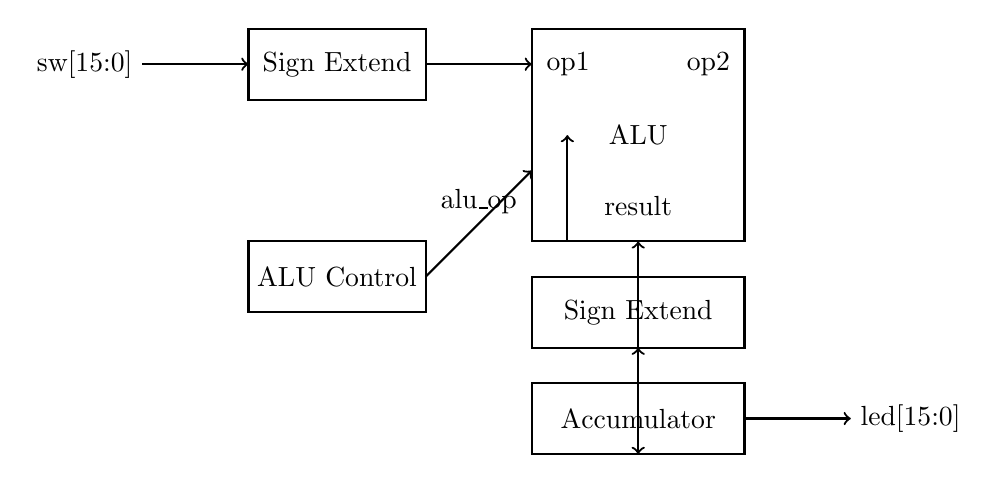
\begin{tikzpicture}[scale=0.9]
    % Sign Extend for switches
    \draw[thick] (0,4) rectangle (2.5,5);
    \node at (1.25,4.5) {Sign Extend};
    \draw[->,thick] (-1.5,4.5) -- (0,4.5);
    \node[left] at (-1.5,4.5) {sw[15:0]};
    
    % ALU
    \draw[thick] (4,2) rectangle (7,5);
    \node at (5.5,3.5) {ALU};
    \node at (5.5,4.5) {op1 \hspace{1cm} op2};
    \node at (5.5,2.5) {result};
    
    % ALU Control
    \draw[thick] (0,1) rectangle (2.5,2);
    \node at (1.25,1.5) {ALU Control};
    \draw[->,thick] (2.5,1.5) -- (4,3);
    \node[above] at (3.25,2.25) {alu\_op};
    
    % Accumulator
    \draw[thick] (4,-1) rectangle (7,0);
    \node at (5.5,-0.5) {Accumulator};
    
    % Sign Extend for accumulator
    \draw[thick] (4,0.5) rectangle (7,1.5);
    \node at (5.5,1) {Sign Extend};
    
    % Connections
    \draw[->,thick] (2.5,4.5) -- (4,4.5);
    \draw[->,thick] (5.5,0) -- (5.5,0.5);
    \draw[->,thick] (5.5,1.5) -- (5.5,2);
    \draw[->,thick] (5.5,2) -- (4.5,2) -- (4.5,3.5);
    \draw[->,thick] (5.5,2) -- (5.5,-1);
    
    % LED output
    \draw[->,thick] (7,-0.5) -- (8.5,-0.5);
    \node[right] at (8.5,-0.5) {led[15:0]};
\end{tikzpicture}
\caption{Διάγραμμα ροής της αριθμομηχανής}
\end{figure}

\subsection{Αποτελέσματα Testbench}

Η αριθμομηχανή ελέγχθηκε με τα ακόλουθα τεστ:

\begin{table}[H]
\centering
\caption{Αποτελέσματα τεστ αριθμομηχανής}
\small
\begin{tabular}{|c|c|c|c|c|c|}
\hline
\textbf{btnl,btnr,btnd} & \textbf{Acc (πριν)} & \textbf{Switches} & \textbf{Λειτουργία} & \textbf{Αναμενόμενο} & \textbf{Αποτέλεσμα} \\
\hline
Reset & xxxx & xxxx & Reset & 0x0000 & PASS \\
0,1,0 & 0x0000 & 0x285a & ADD & 0x285a & PASS \\
1,1,1 & 0x285a & 0x04c8 & XOR & 0x2c92 & PASS \\
0,0,0 & 0x2c92 & 0x0005 & SRL & 0x0164 & PASS \\
1,0,1 & 0x0164 & 0xa085 & NOR & 0x5e1a & PASS \\
1,0,0 & 0x5e1a & 0x07fe & MULT & 0x13cc & PASS \\
0,0,1 & 0x13cc & 0x0004 & SLL & 0x3cc0 & PASS \\
1,1,0 & 0x3cc0 & 0xfa65 & NAND & 0xc7bf & PASS \\
0,1,1 & 0xc7bf & 0xb2e4 & SUB & 0x14db & PASS \\
\hline
\end{tabular}

\justify %stop centering
\subsection{Κυματομορφές Αριθμομηχανής}

\begin{figure}[H]
\centering
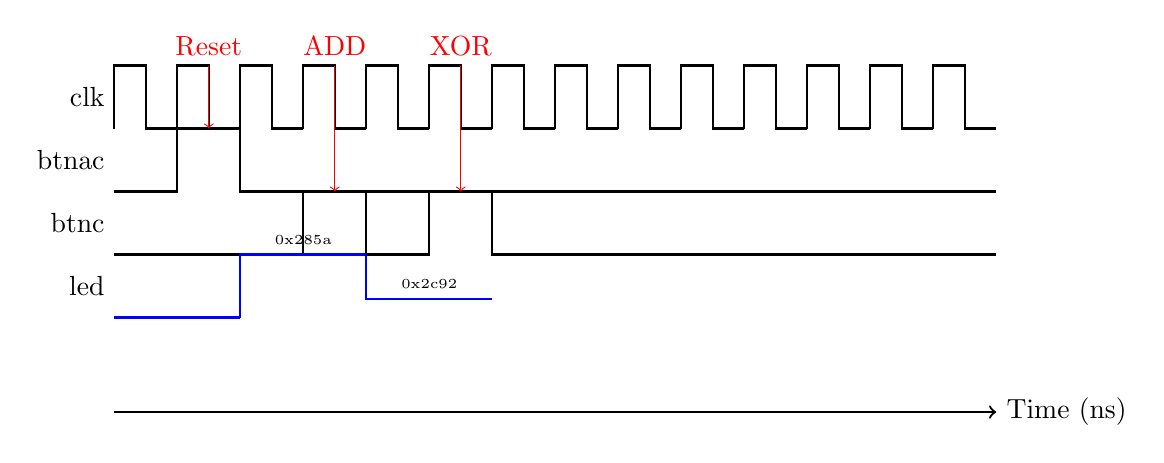
\begin{tikzpicture}[scale=0.8]
    % Time axis
    \draw[->,thick] (0,0) -- (14,0) node[right] {Time (ns)};
    
    % Clock
    \node[left] at (0,5) {clk};
    \foreach \i in {0,1,2,3,4,5,6,7,8,9,10,11,12,13} {
        \draw[thick] (\i,4.5) -- (\i,5.5) -- (\i+0.5,5.5) -- (\i+0.5,4.5) -- (\i+1,4.5);
    }
    
    % btnac
    \node[left] at (0,4) {btnac};
    \draw[thick] (0,3.5) -- (1,3.5) -- (1,4.5) -- (2,4.5) -- (2,3.5) -- (14,3.5);
    
    % btnc
    \node[left] at (0,3) {btnc};
    \draw[thick] (0,2.5) -- (3,2.5) -- (3,3.5) -- (4,3.5) -- (4,2.5) -- 
                 (5,2.5) -- (5,3.5) -- (6,3.5) -- (6,2.5) -- (14,2.5);
    
    % led
    \node[left] at (0,2) {led};
    \draw[thick,blue] (0,1.5) -- (2,1.5);
    \draw[thick,blue] (2,1.5) -- (2,2.5) -- (4,2.5);
    \node[above,font=\tiny] at (3,2.5) {0x285a};
    \draw[thick,blue] (4,2.5) -- (4,1.8) -- (6,1.8);
    \node[above,font=\tiny] at (5,1.8) {0x2c92};
    
    % Annotations
    \draw[<-,red] (1.5,4.5) -- (1.5,5.5) node[above] {Reset};
    \draw[<-,red] (3.5,3.5) -- (3.5,5.5) node[above] {ADD};
    \draw[<-,red] (5.5,3.5) -- (5.5,5.5) node[above] {XOR};
\end{tikzpicture}
\caption{Σχηματική αναπαράσταση κυματομορφών αριθμομηχανής}
\end{figure}

\textbf{Σημείωση:} Για λεπτομερείς κυματομορφές, χρησιμοποιήστε τα αρχεία VCD που παράγονται από τα testbenches στο Playground EDA.

\end{table}